\section{Tor}
\label{sec:tor}

Tor is an implementation of the onion routing architecture model. The
onion routing consists in a technique that provides anonymous
connections over a computer network\cite{goldschlag1999onion}.
%This property is achieved closing the communication data stream through a
%chain of encryption steps. 

%As introduced before, 
Tor is born with the aim to allow people to
improve their privacy and security on the Internet. Its architecture is
based on the Onion Routing model and it's widely used by many user over
the world. Users may be interested on using Tor for different purposes
such as avoiding website tracking, communicating securely over Internet
messaging services, or just web surfing with the access on the services
blocked by their local Internet providers.

The idea behind Tor, and Onion Routing as well, is to protect people
against a common form of Internet surveillance known as "traffic
analysis". Traffic analysis can reveal information about the network
traffic such as the source, destination, size, timing and more of the
analyzed traffic packets. This can be possible even if the packets are
cyphered because the traffic analysis focuses on the header part of the
packets that are in plain text. 

Thus, simply listing between the sender and recipient on the network,
a traffic analysis can be performed. Moreover, spying on multiple parts
of the Internet and using some statistical techniques, some attackers can
track the communications patterns of many different organizations and
individuals.

In the next paragraphs we will discuss more in details about Tor communications 
and the flaws of the model.

\subsection{Tor Internals}
The figure \ref{fig:onion} shows how a
message is cyphered before the communication begins. The communication
source, before sending the message, choses a communication path of nodes
which the keys are known to the sender.
Then the source node is able to create a stack of encryption starting
with the key of the last relay node and then continuing backwards with
the keys of the other relay nodes in the chain. In this way every node
in the communication path can decrypt the package and read the next hop
address. After that the final node receives the message, he can send the
response back to the originator of the data stream. In this phase the response
message is encrypted sequentially by each node in the chain. 
With this method each relay node can gain access to the
previous and the next node addresses only. Anyway the last node of the
Onion Routing path, called exit node, send the message to the end point
as plain text.

\begin{figure}[H]
    \centering
    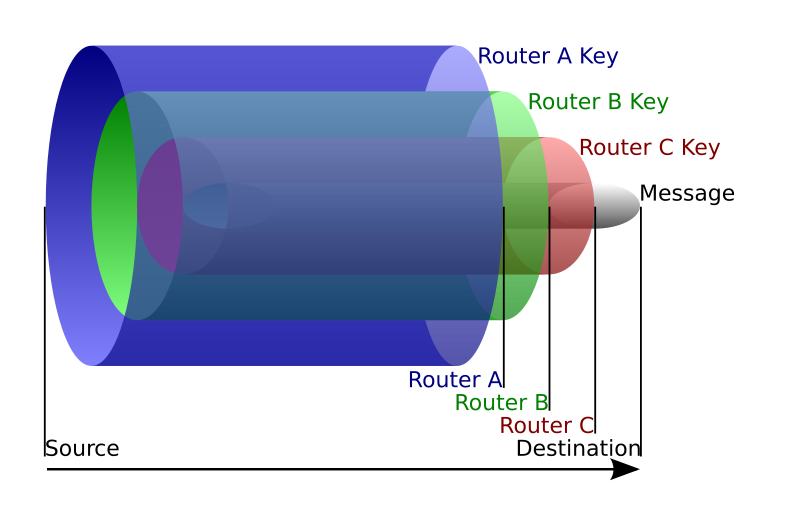
\includegraphics[scale=0.30]{onion.png}
    \caption{Message encryption layers.}
    \label{fig:onion}
    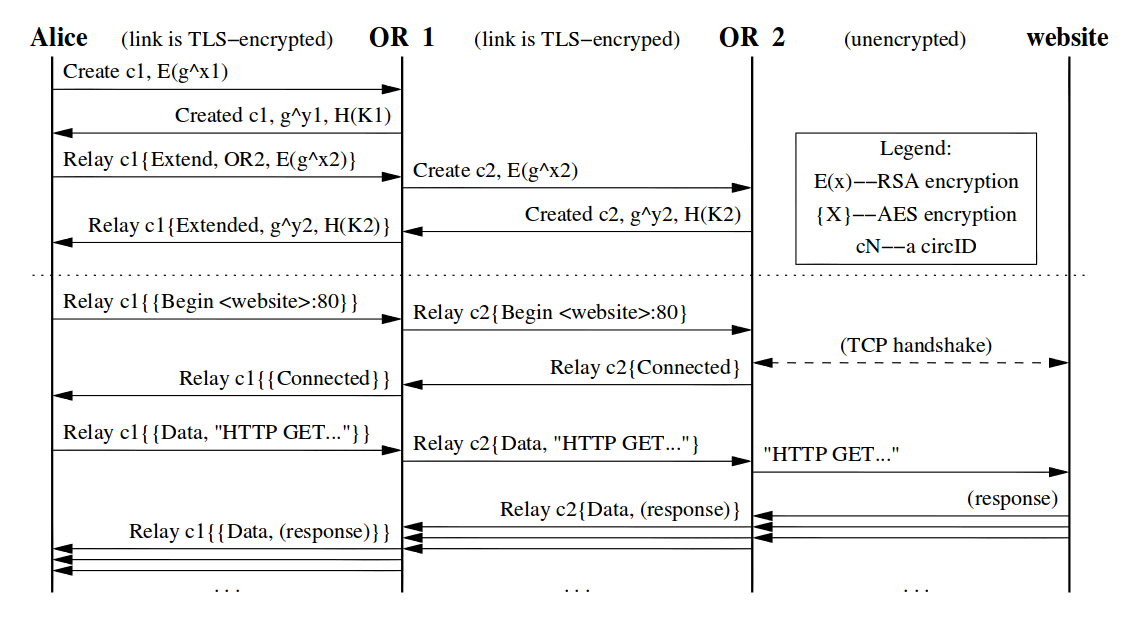
\includegraphics[scale=0.30]{or-communication.png}
    \caption{A two relay Onion Router communication.\cite{dingledine2004tor}}
\end{figure}

\subsection{Tor attacks}
Recent studies showed the existence of different kinds
of possible attacks on the Tor network. 
%TODO ref Recent Attacks On Tor
%TODO Juha Salo
Apart from Side channel attacks \footnote{For example the well known \emph{tor browser attack }.
%CITA WIKIPEDIA
}
we can classify these attacks in
two major families: probabilistic attacks and path selection forcing attacks.
The first ones are based on the data analysis that leak from the network. 
In these cases an attacker that sniff some specific data packets can perform some 
statistical analysis and may be aware of users identity informations.
On the other hand, the path selection forcing attacks are based on some techniques 
able to route the network traffic through a sequence of nodes handled by the attacker.
In our study case we focus on one of the probabilistic attacks: Timing Analysis Attack.
 
\subsubsection{Timing Attack}
As Tor development team states Tor is vulnerable to the timing attack analysis:
\begin{quote}
\emph{``Tor does not provide protection against end-to-end timing attacks[...]''}
\end{quote}
More specifically, an attacker placing between the communication source and the Tor entry node and also between the Tor exit node and the communication destination, can observe the connection time of both end-points and point out their relation.
The attacker can, for example, inject some malware code in the communication source machine or in some
other entities, i.e. a router, on the network segment before the entry node. Similarly, a way to introduce some eavesdropping point into the communication destination could be found by the attacker.

We will focus on how much this kind of attack can be effective on a real network, considering the amount of the resources available to the attacker.
% TODO LINK

